
\de{ĐỀ THI GIỮA HỌC KỲ II NĂM HỌC 2022-2023}{THPT Nguyễn Thái Bình}
\begin{center}
	\textbf{PHẦN 1 - TRẮC NGHIỆM}
\end{center}
\Opensolutionfile{ans}[ans/ans]
%Câu 1...........................
\begin{ex}%[0T9Y2-1]%[Dự án đề kiểm tra HKII NH22-23- Mui Doan]%[THPT Nguyễn Thái Bình]
	Véc-tơ nào dưới đây là một véc-tơ pháp tuyến của $d\colon 2x-3y+20218=0$?
	\choice
	{$\overrightarrow{u}_1=(-3;-2)$}
	{$\overrightarrow{u}_4=(2;-3)$}
	{\True $\overrightarrow{u}_3=(-3;2)$}
	{$\overrightarrow{u}_2=(2;3)$}
	\loigiai{
	$d\colon 2x-3y+2018=0 \Rightarrow \overrightarrow n=(2 ;-3)$ là véc-tơ pháp tuyến của $d$.	
	}
\end{ex}
%Câu 2...........................
\begin{ex}%[0T9Y3-1]%[Dự án đề kiểm tra HKII NH22-23- Mui Doan]%[THPT Nguyễn Thái Bình]
	Tọa độ tâm $I$  của đường tròn $(C)\colon x^2+y^2-4x+2y-1=0$ là
	\choice
	{$I(4;-2)$}
	{$I(-4;2)$}
	{$I(-2;1)$}
	{\True $I(2;-1)$}
	\loigiai{
	Từ phương trình đường tròn ta có $a=2$, $b=-1\Rightarrow I(2 ;-1)$.	
	}
\end{ex}
%Câu 3...........................
\begin{ex}%[0T7B2-1]%[Dự án đề kiểm tra HKII NH22-23- Mui Doan]%[THPT Nguyễn Thái Bình]
	Cho tam thức bậc hai $f(x) = ax^2 + bx + c (a > 0)$ và $f (x)$ có hai nghiệm phân biệt $x_1$, $x_2$ sao cho $x_1 < x_2$. Khi đó $f (x)$ nhận giá trị âm khi $x$ thuộc
	\choice
	{$[x_1;x_2]$} 
	{$(-\infty;x_1)$}
	{\True $(x_1;x_2)$}
	{$(x_2;+\infty)$}
	\loigiai{
	$f(x)$ có $a>0$ và $\Delta>0$ nên suy ra $f(x)$ nhận giá trị âm khi $x \in (x_1 ; x_2)$.	
	}
\end{ex}
%Câu 4...........................
\begin{ex}%[0T9B2-3]%[Dự án đề kiểm tra HKII NH22-23- Mui Doan]%[THPT Nguyễn Thái Bình]
	Xét vị trí tương đối của hai đường thẳng $d_1\colon x-2y+1=0$ và \break$d_2\colon -3x+6y-10=0$.
	\choice
	{Trùng nhau}
	{\True Song song}
	{Vuông góc với nhau}
	{Cắt nhau nhưng không vuông góc nhau}
	\loigiai{
	Ta có $\dfrac{1}{-3}=\dfrac{-2}{6}\ne \dfrac{1}{-10}\Rightarrow$ $d_1$ song song $d_2$.	
	}
\end{ex}
%Câu 5...........................
\begin{ex}%[0T9Y2-1]%[Dự án đề kiểm tra HKII NH22-23- Mui Doan]%[THPT Nguyễn Thái Bình]
	Véc-tơ nào dưới đây là một véc-tơ chỉ phương của đường thẳng đi qua hai điểm $A(3;-1)$, $B(1;-5)$?
	\choice
	{$\overrightarrow{u}_1=(-3;-2)$}
	{\True $\overrightarrow{u}_2=(1;2)$}
	{$\overrightarrow{u}_3=(-3;2)$}
	{$\overrightarrow{u}_4=(2;-3)$}
	\loigiai{
		Ta có $\vec{AB}=(-2;-4)$ là một véc-tơ chỉ phương nên suy ra $\overrightarrow{u}=(1 ; 2)$ cũng là véc-tơ chỉ phương.	
	}
\end{ex}
%Câu 6...........................
\begin{ex}%[0D7B3-2]%[Dự án đề kiểm tra HKII NH22-23- Mui Doan]%[THPT Nguyễn Thái Bình]
	Nghiệm của phương trình $\sqrt{8-x^2}=\sqrt{x+2}$ là
	\choice
	{$x=-2$}
	{\True $x=2$}
	{$x=-3$}
	{$\hoac{&x=2\\&x=-3}$}
	\loigiai{
	Ta có \begin{eqnarray*}
		\sqrt{8-x^2}=\sqrt{x+2}&\Rightarrow& 8-x^2=x+2\\
		&\Rightarrow & x^2+x-6=0 \Rightarrow \hoac{& x=2 \\ & x=-3. }
	\end{eqnarray*}
	Thay lần lượt $x=2$ và $x=-3$ vào phương trình đã cho ta thấy $x=2$ là nghiệm.	
	}
\end{ex}
%Câu 7...........................
\begin{ex}%[0T9B3-1]%[Dự án đề kiểm tra HKII NH22-23- Mui Doan]%[THPT Nguyễn Thái Bình]
	Phương trình nào sau đây là phương trình của một đường tròn?
	\choice
	{$x^2-y^2+6x-4y+2=0$}
	{$x^2+y^2+2x-6y+20=0$}
	{\True $x^2+y^2+2x-4y-1=0$}
	{$x^2+2y^2+6x-10y+45=0$}
	\loigiai{
		Từ phương trình $x^2+y^2+2x-4y-1=0$ ta có $a=-1$, $b=2$, $c=-1$.\\
	Suy ra $a^2+b^2-c=1+4+1=6>0$ nên đây là phương trình đường tròn.	
	}
\end{ex}
%Câu 8...........................
\begin{ex}%[0T7B3-2]%[Dự án đề kiểm tra HKII NH22-23- Mui Doan]%[THPT Nguyễn Thái Bình]
	Phương trình $\sqrt{4x^2-3}=x$ có nghiệm là
	\choice
	{$x=-1$}
	{$x=2$}
	{\True $x=1$}
	{$x=1$ hoặc $x=-1$}
	\loigiai
	{
		Ta có $\sqrt{4x^2-3}=x\Rightarrow 3x^2-3=0\Rightarrow x^2=1\Rightarrow \hoac{& x=1 \\ &x=-1. }$\\
		Thay lần lượt $x=1$ và $x=-1$ vào phương trình đã cho ta thấy $x=1$ là nghiệm.
	}
\end{ex}
%Câu 9...........................
\begin{ex}%[0T9Y1-1]%[Dự án đề kiểm tra HKII NH22-23- Mui Doan]%[THPT Nguyễn Thái Bình]
	Cho $\vec{a}=(-1 ; 2), \vec{b}=(5 ;-7)$. Tọa độ của véc-tơ $\vec{a}-\vec{b}$ là
	\choice
	{ $(6 ;-9)$}
	{ $(4 ;-5)$}
	{\True $(-6 ; 9)$}
	{ $(-5 ;-14)$}
	\loigiai
	{
		Ta có $\vec{a}-\vec{b}=(-6 ; 9)$.
	}
\end{ex}
%Câu 10...........................
\begin{ex}%[0T7B2-1]%[Dự án đề kiểm tra HKII NH22-23- Mui Doan]%[THPT Nguyễn Thái Bình]
	Tập nghiệm của bất phương trình $x^2+9>6x$ là
	\choice
	{\True $\mathbb{R} \setminus \{3\}$}
	{$\mathbb{R}$}
	{ $(3 ;+\infty)$}
	{ $(-\infty ; 3)$}
	\loigiai
	{
		Ta có $x^2+9>6x \Leftrightarrow x^2-6x+9>0\Leftrightarrow (x-3)^2>0\Leftrightarrow x\ne 3$.\\
		Vậy tập nghiệm của bất phương trình là $S=\mathbb{R} \setminus \{3\}$
	}
\end{ex}
%Câu 11...........................
\begin{ex}%[0T7B2-1]%[Dự án đề kiểm tra HKII NH22-23- Mui Doan]%[THPT Nguyễn Thái Bình]
	Tập nghiệm của bất phương trình $-x^2+5x-6>0$ là
	\choice
	{ $(2 ;+\infty)$}
	{ $(3 ;+\infty)$}
	{ \True $(2 ; 3)$}
	{ $(-\infty ; 2)$}
	\loigiai
	{
		Ta có  $-x^2+5x-6>0 \Leftrightarrow 2<x<3$.
	}
\end{ex}
%Câu 12...........................
\begin{ex}%[0T7Y2-1]%[Dự án đề kiểm tra HKII NH22-23- Mui Doan]%[THPT Nguyễn Thái Bình]
	Trong các bất phương trình sau, bất phương trình nào là bất phương trình bậc hai một ẩn?
	\choice
	{ \True $x^2+x-1 \leq 0$}
	{$x^2+x y-1>0$}
	{$x^3+x-1<0$}
	{$x^2+2 y+1>0$}
	\loigiai
	{
		$x^2+x-1 \leq 0$ là một  bất phương trình bậc hai một ẩn.
	}
\end{ex}
%Câu 13...........................
\begin{ex}%[0T9Y3-1]%[Dự án đề kiểm tra HKII NH22-23- Mui Doan]%[THPT Nguyễn Thái Bình]
	Tọa độ tâm $I$ và bán kính $R$ của đường tròn $(C) \colon (x+1)^2+y^2=8$ là
	\choice
	{$I(-1 ; 0), R=8$}
	{$I(-1 ; 0), R=64$}
	{ \True $I(-1 ; 0), R=2 \sqrt{2}$}
	{$I(1 ; 0), R=2 \sqrt{2}$}
	\loigiai
	{
		Từ phương trình đường tròn ta có $a=-1$, $b=0$ và $R=2 \sqrt{2}$.
	}
\end{ex}
%Câu 14...........................
\begin{ex}%[0T7B3-2]%[Dự án đề kiểm tra HKII NH22-23- Mui Doan]%[THPT Nguyễn Thái Bình]
	Tập nghiệm của phương trình $\dfrac{x^2-5x}{\sqrt{x-2}}=-\dfrac{4}{\sqrt{x-2}}$ là
	\choice
	{ \True $S=\{4\}$}
	{ $S=\{1 ; 4\}$}
	{$S=\{1\}$}
	{ $S=\varnothing$}
	\loigiai
	{
		Điều kiện của phương trình: $x>2$.\\
		$\dfrac{x^2-5x}{\sqrt{x-2}}=-\dfrac{4}{\sqrt{x-2}}\Rightarrow x^2-5x+4=0\Leftrightarrow\hoac{& x=1 \text{ (loại)} \\ & x=4 \text{ (nhận)}.}$\\
		Vậy tập nghiệm $S=\{4\}$.
	}
\end{ex}
%Câu 15...........................
\begin{ex}%[0T7Y1-1]%[Dự án đề kiểm tra HKII NH22-23- Mui Doan]%[THPT Nguyễn Thái Bình]
	Xác định tất cả các giá trị của $m$ để đa thức $(m-1)x^2+2(m-1) x+4$ là tam thức bậc hai.
	\choice
	{$m=1$}
	{ \True $m \neq 1$}
	{ $m \neq-1$}
	{ $m<2$}
	\loigiai
	{
		$(m-1)x^2+2(m-1) x+4$ là tam thức bậc hai khi $m-1\ne 0\Leftrightarrow m \ne 1$.
	}
\end{ex}
%Câu 16...........................
\begin{ex}%[0T9Y1-1]%[Dự án đề kiểm tra HKII NH22-23- Mui Doan]%[THPT Nguyễn Thái Bình]
	Trong mặt phẳng tọa độ $Oxy$, tọa độ của véc-tơ $\vec{j}-2 \vec{i}$ là
	\choice
	{ $(2 ;-1)$}
	{ \True $(-2 ; 1)$}
	{ $(-1 ; 2)$}
	{ $(1 ;-2)$}
	\loigiai
	{
		Ta có $\vec{j}-2\vec{i}=(-2 ; 1)$.
	}
\end{ex}
%Câu 17...........................
\begin{ex}%[0T9B3-2]%[Dự án đề kiểm tra HKII NH22-23- Mui Doan]%[THPT Nguyễn Thái Bình]
	Trong mặt phẳng $Oxy$, đường tròn có tâm $I(1 ;-2)$, bán kính $R=2$ có phương trình là
	\choice
	{ $(x+1)^2+(y-2)^2=4$}
	{$(x-1)^2+(y+2)^2=2$}
	{$(x+1)^2+(y-2)^2=2$}
	{ \True $(x-1)^2+(y+2)^2=4$}
	\loigiai
	{
		Đường tròn có tâm $I(1 ;-2)$, bán kính $R=2$ có phương trình là $(x-1)^2+(y+2)^2=4$.
	}
\end{ex}
%Câu 18...........................
\begin{ex}%[0T7B1-1]%[Dự án đề kiểm tra HKII NH22-23- Mui Doan]%[THPT Nguyễn Thái Bình]
	Bất phương trình nào sau đây có tập nghiệm là $\mathbb{R}$ ?
	\choice
	{ $-3x^2+x-1 \geq 0$}
	{$-3x^2+x-1>0$}
	{ $3x^2+x-1 \leq 0$}
	{\True $-3x^2+x-1<0$}
	\loigiai
	{
		Xét bất phương trình $-3x^2+x-1<0$. \\
		Tam thức $f(x)=-3x^2+x-1$ có $a=-3<0$ và $\Delta = -11<0$ nên suy ra $f(x)<0~\forall x \in \mathbb{R}$.\\
		Do đó $-3x^2+x-1<0$ tập nghiệm là $\mathbb{R}$.
	}
\end{ex}
%Câu 19...........................
\begin{ex}%[0T7B3-2]%[Dự án đề kiểm tra HKII NH22-23- Mui Doan]%[THPT Nguyễn Thái Bình]
	Cho phương trình $\sqrt{x^2+3}=\sqrt{2x+6}$. Khẳng định nào sau đây \textbf{sai}?
	\choice
	{ Các nghiệm của phương trình đã cho đều lớn hơn $-2$}
	{ Phương trình có hai nghiệm trái dấu}
	{\True Tích các nghiệm của phương trình đã cho là $-5$}
	{Tổng các nghiệm của phương trình đã cho là $2$}
	\loigiai
	{
		Ta có $\sqrt{x^2+3}=\sqrt{2x+6}\Rightarrow x^2-2x-3=0\Rightarrow \hoac{& x=-1 \\ & x=3.}$\\
		Thay lần lượt $x=-1$ và $x=3$ vào phương trình đã cho ta thấy $x=-1$ và $x=3$ là nghiệm.\\
		Suy ra tích các nghiệm của phương trình đã cho là $-5$ là sai. 
	}
\end{ex}
%Câu 20...........................
\begin{ex}%[0T3K1-3]%[Dự án đề kiểm tra HKII NH22-23- Mui Doan]%[THPT Nguyễn Thái Bình]
	\immini
	{
		Cho hàm số bậc hai $y=f(x)$ có đồ thị như hình vẽ $f(x)$ nhận giá trị dương khi $x$ thuộc
	}
	{
		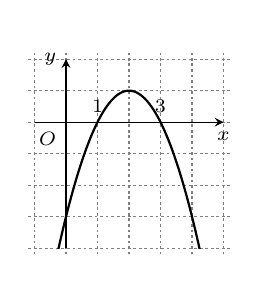
\begin{tikzpicture}[>=stealth,x=1cm,y=1cm,scale=0.4]
			\def\a{-1} % Hệ số a phải khác 0
			\def\b{4}
			\def\c{-3}
			\draw[color=gray,dash pattern=on 1pt off 1pt,xstep=1.0cm,ystep=1.0cm] (-1.2,-4.2) grid (5.2,2.2);
			\draw[->] (-1,0) -- (5,0) node[below] {\scriptsize $x$};
			\draw[->] (0,-4) -- (0,2) node[left] {\scriptsize $y$};
			\draw (0,0)node[below left]{\scriptsize $O$};
			\clip (-1,-4)rectangle(5,3);
			\draw[thick,samples=150,smooth,domain=-5:5] plot(\x,{\a*(\x)^2+(\b)*\x+(\c)});
			\foreach \x in {1,3}\draw (\x,0) node[above]{\scriptsize $\x$};
		\end{tikzpicture}   
	}
	\choice
	{$[1 ; 3]$}
	{\True $(1 ; 3)$}
	{$(3 ;+\infty)$}
	{$(-\infty ; 1)$}
	\loigiai
	{
		Dựa vào đồ thị ta suy ra $f(x)> 0$ khi $x\in (1;3)$.
	}
\end{ex}

\begin{ex}%[Dự án đề kiểm tra GHKII NH22-23- Nguyễn Tài Tuệ]%[0T9Y1-2]
	Trong mặt phẳng tọa độ $O x y$, cho $A(5 ; 2)$, $B(3 ; 5)$. Tọa độ của véc-tơ $\overrightarrow{B A}$ là
	\choice
	{\True $(-2 ; 3)$}
	{$(2 ;-3)$}
	{$(3 ;-2)$}
	{$(-3 ; 2)$}
	\loigiai{
		Ta có $ \vec{BA} =(-2;3) $.
	}
\end{ex}

\begin{ex}%[Dự án đề kiểm tra GHKII NH22-23- Nguyễn Tài Tuệ]%[0T7B3-2]
	Số nghiệm của phương trình $\sqrt{-x^2+4 x}=2 x-2$ là 
	\choice
	{$ 2  $}
	{$ 3  $}
	{$ 0  $}
	{\True $ 1  $}
	\loigiai{
		Ta có 
		\begin{eqnarray*}
			&&\sqrt{-x^2+4 x}=2 x-2\\
			&\Rightarrow& -x^2+4x=(2x-2)^2\\
			&\Rightarrow& -5x^2+12x-4=0\\
			&\Rightarrow& \hoac{&x=2\\&x=\dfrac{2}{5}.}
		\end{eqnarray*}
		Thử lần lượt $ x=2 $ và $ x=\dfrac{2}{5} $ vào phương trình đã cho ta thấy $ x=2 $ thỏa mãn.\\
		Vậy phương trình đã cho có một nghiệm duy nhất.
	}
\end{ex}

\begin{ex}%[Dự án đề kiểm tra GHKII NH22-23- Nguyễn Tài Tuệ]%[0T7Y1-1]
	\immini{	Cho hàm số bậc hai $\mathrm{f}(x )$ có đồ thị như hình bên. Tập nghiệm của bất phương trình $\mathrm{f}(x ) \geq 0$ là 
		\choice
		{$(-\infty ;-1) \cup(5 ;+\infty)$ }
		{$(-1 ; 5)$ }
		{$[-1 ; 5]$}
		{\True $(-\infty ;-1] \cup[5 ;+\infty)$ }}{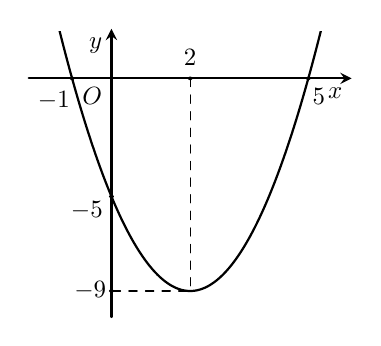
\begin{tikzpicture}[line join=round, line cap=round,>=stealth,thick,xscale=0.5,yscale=0.3]
			\tikzset{every node/.style={scale=0.9}}
			\draw[->] (-2.1,0)--(6.1,0) node[below left] {$x$};
			\draw[->] (0,-10.1)--(0,2.1) node[below left] {$y$};
			\draw (0,0) node [below left] {$O$};
			\draw[dashed,thin](2,0)--(2,-9)--(0,-9);
			\begin{scope}
				\clip (-2,-10) rectangle (6,2);
				\draw[samples=200,domain=-1.5:5.5,smooth,variable=\x] plot (\x,{1*(\x)^2+-4*(\x)+-5});
			\end{scope}
			\draw[fill=black] (-1,0) circle (1pt) node[shift={(-130:0.4)}]{$ -1$};
			\draw[fill=black] (5,0) circle (1pt) node[shift={(-60:0.3)}]{$ 5$};
			\draw[fill=black] (2,0) circle (1pt) node[shift={(90:0.3)}]{$ 2$};
			\draw[fill=black] (0,-5) circle (1pt) node[shift={(-150:0.4)}]{$ -5$};
			\draw[fill=black] (0,-9) circle (1pt) node[shift={(-180:0.3)}]{$ -9$};
	\end{tikzpicture}}
	\loigiai{
		Dựa vào đồ thị ta thấy $ f(x)\ge 0\Leftrightarrow \hoac{&x\le -1\\&x\ge 5.} $ 
	}
\end{ex}

\begin{ex}%[Dự án đề kiểm tra GHKII NH22-23- Nguyễn Tài Tuệ]%[0T9B2-2]
	Trong mặt phẳng $Oxy$, phương trình tham số của đường thẳng $d$ đi qua điểm $A(-1 ; 2)$ và song song với đường thẳng $\Delta: 3 x-13 y+1=0$ là 
	\choice
	{$\heva{&x=-1+13 t \\ &y=2+3 t}$}
	{$\heva{&x=1+13 t \\ &y=-2+3 t}$}
	{$\heva{&x=-1-13 t \\& y=2+3 t}$}
	{$\heva{&x=1+3 t \\ &y=2-13 t}$}
	\loigiai{
		Một véc-tơ chỉ phương của đường thẳng $ \Delta $ là $ \vec{u}_{\Delta} =(13;3) $.\\
		Đường thẳng $ d $ song song với $ \Delta $ nên $ d $ có véc-tơ chỉ phương là $ \vec{u}_{d}=\vec{u}_{\Delta} =(13;3) $.\\
		Phương trình tham số của đường thẳng $ d $ đi qua $ A(-1;2) $ và song song với đường thẳng $ \Delta  $ là $ \heva{&x=-1+13t\\&y=2+3t.} $
	}
\end{ex}

\begin{ex}%[Dự án đề kiểm tra GHKII NH22-23- Nguyễn Tài Tuệ]%[0T9B2-2]
	Trong mặt phẳng $Oxy$, phương trình nào sau đây là phương trình tổng quát của đường thẳng $d\colon \heva{&x=3-5 t \\&y=1+4 t}$?
	\choice
	{\True $4 x+5 y-17=0$}
	{$4 x-5 y+17=0$}
	{$4 x+5 y+17=0$}
	{$4 x-5 y-17=0$}
	\loigiai{
		Đường thẳng $ d $ đi qua điểm $ (3;1) $ và có véc-tơ pháp tuyến là $ \vec{n}=(4;5) $ nên có phương trình $$ 4(x-3)+5(y-1)=0\Leftrightarrow 4x+5y-17=0 .$$
	}
\end{ex}

\begin{ex}%[Dự án đề kiểm tra GHKII NH22-23- Nguyễn Tài Tuệ]%[0T7B1-1]
	Bảng xét dấu sau đây là của tam thức bậc hai nào?
	\begin{center}
		
\begin{tikzpicture}
			\tkzTabInit[lgt=1.2,espcl=2]
			{$x$ /1, $f(x)$ /1}
			{$-\infty$,$-6$,$+\infty$}
			\tkzTabLine{ ,+,z,+, }
		\end{tikzpicture}
	\end{center}
	\choice
	{$f(x)=x^2-12 x+36$}
	{$f(x)=-x^2+12 x+36$}
	{$f(x)=x^2-36$}
	{\True $f(x)=x^2+12 x+36$}
	\loigiai{
		Từ bảng biến thiên ta thấy tam thức $ f(x) $ có $ \heva{&a>0\\&\Delta = 0\\&x_1=x_2=-6.} $\\
		Do đó chỉ có tam thức $f(x)=x^2+12 x+36$ thỏa mãn.
	}
\end{ex}

\begin{ex}%[Dự án đề kiểm tra GHKII NH22-23- Nguyễn Tài Tuệ]%[0T9B3-2]
	Trong mặt phẳng $Oxy$, đường tròn $(C)$ có tâm $I(-2 ; 3)$ và đi qua $M(2 ;-3)$ có phương trình là:
	\choice
	{$(x+2)^2+(y-3)^2=\sqrt{52}$}
	{$(x-2)^2+(y+3)^2=52$}
	{$x^2+y^2+4 x-6 y-57=0$}
	{\True $x^2+y^2+4 x-6 y-39=0$}
	\loigiai{
		Bán kính đường tròn $ R=IM=\sqrt{4^2+6^2} =\sqrt{52}.$\\
		Đường tròn $(C)$ có tâm $I(-2 ; 3)$ và đi qua $M(2 ;-3)$ có phương trình là $$ (x+2)^2+(y-3)^2=52 \Leftrightarrow x^2+y^2+4x-6y-39=0. $$
	}
\end{ex}

\begin{ex}%[Dự án đề kiểm tra GHKII NH22-23- Nguyễn Tài Tuệ]%[0T9Y1-2]
	Trong mặt phẳng Oxy, cho $\vec{a}=(1 ; 2), \vec{b}=(-5 ; 2)$. Tọa độ của véc-tơ $\vec{c}=2 \vec{a}-\vec{b}$ là
	\choice
	{$(7 ; 2)$}
	{$(-7 ;-2)$}
	{$(-7 ; 2)$}
	{$(7 ;-2)$}
	\loigiai{
		Ta có $\vec{c}=2 \vec{a}-\vec{b}= (7;2)$.
	}
\end{ex}

\begin{ex}%[Dự án đề kiểm tra GHKII NH22-23- Nguyễn Tài Tuệ]%[0T7B2-1]
	Tam thức bậc hai $f(x)=x^2-m x-m$  luôn dương với mọi $x \in \mathbb{R}$ khi 
	\choice
	{$-4 \leq m \leq 0$}
	{\True $-4<m<0$}
	{$m<-4$ hoặc $m>0$}
	{$m \leq-4$ hoặc $m \geq 0$}
	\loigiai{
		Tam thức bậc hai $f(x)=x^2-m x-m$  luôn dương với mọi $x \in \mathbb{R}$ khi và chỉ khi $$ \heva{&a=1>0\\&\Delta <0}\Leftrightarrow m^2+4m<0\Leftrightarrow -4<m<0 .$$
	}
\end{ex}

\begin{ex}%[Dự án đề kiểm tra GHKII NH22-23- Nguyễn Tài Tuệ]%[0T7B3-2]
	Tổng các nghiệm của phương trình $(x-2) \sqrt{2 x+7}=x^2-4$ bằng 
	\choice
	{$ 1  $}
	{$ 0  $}
	{$ 3  $}
	{\True $ 2 $}
	\loigiai{
		\begin{eqnarray*}
			&&(x-2) \sqrt{2 x+7}=x^2-4\\
			&\Rightarrow& (x-2)\left(\sqrt{2x+7} -(x+2)\right)=0\\
			&\Rightarrow& \hoac{&x=2\\&\sqrt{2x+7} = x+2 } \\
			&\Rightarrow& \hoac{&x=2\\&2x+7=x^2+4x+4}\\
			&\Rightarrow& \hoac{&x=2\\&x^2+2x-3=0}\\
			&\Rightarrow& \hoac{&x=2\\&x=1\\&x=-3.}
		\end{eqnarray*}
		Thử lại ta thấy $ x=2 $ và $ x=1 $ là nghiệm của phương trình.
	}
\end{ex}

\begin{ex}%[Dự án đề kiểm tra GHKII NH22-23- Nguyễn Tài Tuệ]%[0T7T3-2]
	\immini{
		Cổng Arch tại thành phố St Louis của Mỹ có hình dạng là một parabol. Biết khoảng cách giữa hai chân cổng bằng $162\text {m}$. Trên thành cổng, tại vị trí có độ cao $43\text {m}$ so với mặt đất, người ta thả một sợi dây chạm đất. Vị trí chạm đất của đầu sợi dây này cách chân cổng A một đoạn $10\text {m}$. Giả sử các số liệu trên là chính xác. Hãy tính độ cao của cổng Arch.			 		
		\choice
		{$185,6$ m}
		{$ 185,5 $ m}
		{$158,6 $ m}
		{$158,5 $ m}}{
		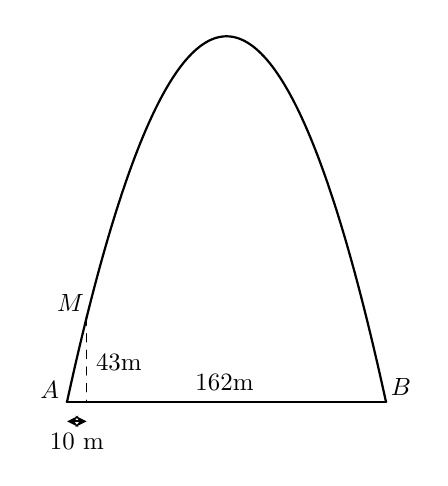
\begin{tikzpicture}[line join=round, line cap=round,>=stealth,thick,scale=0.5]
			\tikzset{every node/.style={scale=0.9}}
			\coordinate (M) at (0.5,2.15);
			\coordinate (A) at (0,0);
			\coordinate (B) at (8.1,0);
			\coordinate (C) at (0.5,0);
			\begin{scope}
				\clip (-1,-1) rectangle (8.5,9.5);
				\draw[samples=200,domain=0:8.1,smooth,variable=\x] plot (\x,{-43/76*(\x)^2+3483/760*(\x)+0});
			\end{scope}
			\draw[dashed,thin] (M)--(C);
			\draw (A)--(B);
			\draw[dashed,<->] (0,-0.5)--(0.5,-0.5) node at (0.25,-1) {$10$ m};
			\foreach \p/\r in {M/140,B/45, A/145}
			\fill (\p) circle (1.0pt) node[shift={(\r:3mm)}]{$\p$};
			\node at (.5,1)[right] {$43$m}; \node at (4,0.5) {$162$m};
	\end{tikzpicture}}
	\loigiai {
	\immini{	Chọn hệ trục tọa độ $Oxy$ như hình vẽ bên.\\
		Phương trình Parabol $\left(P\right)$ có dạng $ y=a{x^2}+bx+c$.\\
		Parabol $\left(P\right)$ đi qua điểm $A\left(0;0\right)$, $B\left(162;0\right)$, $M\left(10;43\right)$ nên ta có
		$$\heva{ &c=0\\ &{162^2}a+162b+c=0\\ &{10^2}a+10b+c=43} \Leftrightarrow \heva{ &c=0\\ &a=-\dfrac{43}{1520}\\ &b=\dfrac{3483}{760}.}$$
		Suy ra $\left(P\right)\colon y=-\dfrac{43}{1520}{x^2}+\dfrac{3483}{760}x$.\\
		Do đó chiều cao của cổng là $ h=-\dfrac{\Delta  }{4a}$$=-\dfrac{{b^2}-4ac}{4a}$$\approx 185{,}6$ m.
	}
	{
		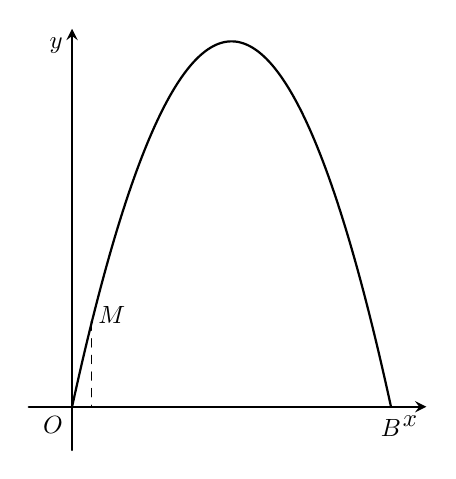
\begin{tikzpicture}[line join=round, line cap=round,>=stealth,thick,scale=0.5]
	\tikzset{every node/.style={scale=0.9}}
	\draw[->] (-1.1,0)--(9,0) node[below left] {$x$};
	\draw[->] (0,-1.1)--(0,9.6) node[below left] {$y$};
	\draw (0,0) node [below left] {$O$};
	\coordinate (M) at (0.5,2.15);
	\coordinate (B) at (8.1,0);
	\coordinate (C) at (0.5,0);
	\begin{scope}
		\clip (-1,-1) rectangle (8.5,9.5);
		\draw[samples=200,domain=0:8.1,smooth,variable=\x] plot (\x,{-43/76*(\x)^2+3483/760*(\x)+0});
	\end{scope}
	\draw[dashed,thin] (M)--(C);
	\foreach \p/\r in {M/20,B/-90}
	\fill (\p) circle (1.0pt) node[shift={(\r:3mm)}]{$\p$};
\end{tikzpicture}	
}
}
\end{ex}

\begin{ex}%[Dự án đề kiểm tra GHKII NH22-23- Nguyễn Tài Tuệ]%[0T9B2-2]
	Trong mặt phẳng với hệ tọa độ $O x y$, cho tam giác $A B C$ có $A(2;-1), B(4; 5)$ và $C(-3; 2)$. Lập phương trình đường cao của tam giác $A B C$ kẻ từ $B$.
	\choice
	{$3 x+5 y-20=0$}
	{$3 x-5 y-13=0$}
	{$5 x-3 y+5=0$}
	{\True $5 x-3 y-5=0$}
	\loigiai{
		Ta có $ \vec{AC}=(-5;3) $, nên phương trình đường cao $ BH $ là $$ -5(x-4)+3(y-5)=0\Leftrightarrow 5x -3y-5=0.$$
	}
\end{ex}

\begin{ex}%[Dự án đề kiểm tra GHKII NH22-23- Nguyễn Tài Tuệ]%[0T9B2-2]
	Trong mặt phẳng $Oxy$, cho $\triangle A B C$ có $A(1 ; 1)$, $B(0 ;-2)$, $C(4 ; 2)$. Viết phương trình tổng quát của đường trung tuyến $A M$ của tam giác $A B C$.
	\choice
	{\True $x+y-2=0$}
	{$x+y+2=0$}
	{$x-y-2=0$}
	{$x-y+2=0$}
	\loigiai{
		Trung điểm của $ BC $ là $ M(2;0) $ và $ \vec{AM}=(1;-1) $ nên véc-tơ pháp tuyến của đường thẳng $ AM $ là $ \vec{n}=(1;1) $.\\
		Do đó phương trình đường trung tuyến $ AM $ có phương trình $$ 1(x-1)+1(y-1)=0\Leftrightarrow x+y-2=0 .$$
	}
\end{ex}

\begin{ex}%[Dự án đề kiểm tra GHKII NH22-23- Nguyễn Tài Tuệ]%[0T9B3-2]
	Trong mặt phẳng $Oxy$, đường tròn đường kính $A B$ với $A(3;-1)$, $B(1 ;-5)$ có phương trình là 
	\choice
	{\True $(x-2)^2+(y+3)^2=5$}
	{$(x+1)^2+(y+2)^2=17$}
	{$(x-2)^2+(y+3)^2=\sqrt{5}$}
	{$(x+2)^2+(y-3)^2=5$}
	\loigiai{
		Trung điểm của  $AB  $ là $ I(2;-3) $ và $ IA=\sqrt{1^2+2^2}=\sqrt{5} $.\\
		Phương trình đường tròn đường kính $ AB $ nhận $ I $ là tâm và bán kính $R=IA $ có phương trình $ (x-2)^2+(y+3)^2=5 $.
	}
\end{ex}

\begin{ex}%[Dự án đề kiểm tra GHKII NH22-23- Nguyễn Tài Tuệ]%[0T7T3-2]
	\immini{Hai xe chuyển động trên hai đường thẳng cắt nhau tạo thành một góc $60^{\circ}$. Xe thứ nhất chuyển động với tốc độ $40$ km/h, xe thứ hai chuyển động với tốc độ $30 \mathrm{~km}/ \mathrm{h}$. Ở thời điểm ban đầu, hai xe cách giao điểm $O$ các khoảng lần lượt là $30 \mathrm{~km}$ và $40 \mathrm{~km}$ (hình vẽ). Hỏi sau bao lâu thì khoảng cách hai xe là $20 \mathrm{~km}$ (làm tròn kết quả đến hàng phần trăm)?
		\choice
		{$2,12 $ h}
		{\True $1,19 $ h}
		{$1,18 $ h}
		{$1,23 $ h}}{
		\begin{tikzpicture}[scale=1,line cap=round,line join=round,font=\footnotesize,>=stealth]
			\clip (-0.5,-0.5) rectangle (4.5,4.9);
			\path
			(-2,0) coordinate (m)
			(5,0) coordinate (n)
			(-1,-2) coordinate (m')
			(3,6) coordinate (n')
			(intersection of m--n and m'--n') coordinate (O)
			($ (O)!3/4!(n) $) coordinate (B)
			($ (O)!2/4!(n) $) coordinate (B')
			($ (O)!3/4!(n') $) coordinate (A)
			($ (O)!2/4!(n') $) coordinate (A')
			;
			
			
			\draw (m)--(n) (m')--(n');
			\draw[->,thick,red] (A)--(A') node[pos=0.5,sloped,above]{$ \vec{v}_1 $};
			\draw[->,thick,red] (B)--(B') node[pos=0.5,sloped,above]{$ \vec{v}_2 $};
			\foreach \p/\g in {O/110,B/-110,B'/-110,A/110,A'/150} \draw[fill] (\p) circle(.5pt)node [shift={(\g:.3)}] {$\p$};
			
			
			\draw pic[draw,angle radius=5mm,angle eccentricity=1.5] {angle = B'--O--A'} node[shift={(30:0.9)}] {$ 60^\circ $};
		\end{tikzpicture}
	}
	\loigiai{
		Gọi $ x $  là thời gian di chuyển mà hai xe cách nhau $ 20 $ km.\\
		Quãng đường xe thứ nhất di chuyển trong thời gian $ x $ h là $ 40x $ km, khi đó cách giao điểm $ O $ là $ 30-40x $ km.\\
		Quãng đường xe thứ hai di chuyển trong thời gian $ x $ h là $ 30x $ km, khi đó cách giao điểm $ O $ là $ 40-30x $ km.\\
		Áp dụng định lí cô-sin vào tam giác $ OA'B' $ ta có
		\begin{eqnarray*}
			&&A'B'^2=OA'^2+OB'^2 -2\cdot OA'\cdot OB' \cos 60^\circ\\
			&\Leftrightarrow& 20^2=(30-40x)^2+(40-30x)^2-(30-40x)(40-30x)\\
			& \Leftrightarrow& 1300 x^2-2300 x+900=0 \Leftrightarrow \hoac{& x\approx 1,19\\&x\approx 0,58.} 
		\end{eqnarray*}
		
	}
\end{ex}

\begin{ex}%[Dự án đề kiểm tra GHKII NH22-23- Nguyễn Tài Tuệ]%[0T9B1-3]
	Trong mặt phẳng $Oxy$, cho $M(2 ; 0)$, $N(2 ; 2)$, $P(-1 ; 3)$ lần lượt là trung điểm các cạnh $BC, CA, AB$ của $\triangle A B C$. Tọa độ điểm $B$ là:
	\choice
	{$(1 ; 1)$}
	{$(-1 ;-1)$}
	{$(1 ;-1)$}
	{$(-1 ; 1)$}
	\loigiai{
		\immini
		{
			Ta có $ BMNP $ là hình bình hành nên \\ $ \vec{PB} =\vec{NM}\Leftrightarrow \heva{&x_B+1=0\\&y_B-3=-2}\Leftrightarrow \heva{&x_B=-1\\&y_B=1.}$
		}
		{
			\begin{tikzpicture}[scale =0.6]
				%		\draw[gray] (-5,-5) grid (5,5);
				\path
				(0,0) coordinate (O)
				(2,0) coordinate (M)
				(2,2) coordinate (N)
				(-1,3) coordinate (P)
				($ (P)+(N)-(M) $) coordinate (A)
				($ (P)+(M)-(N) $) coordinate (B)
				($ (N)+(M)-(P) $) coordinate (C)
				;
				\draw (A)--(B)--(C)--cycle (M)--(N)--(P);
				\foreach \p/\g in {A/90,B/180,C/-90,M/-90,N/60,P/180} \draw[fill] (\p) circle(.5pt)node [shift={(\g:.3)}] {$\p$};
			\end{tikzpicture}
		}	
	}
\end{ex}

\begin{ex}%[Dự án đề kiểm tra GHKII NH22-23- Nguyễn Tài Tuệ]%[0T9B3-3]
	Trong mặt phẳng $Oxy$, với những giá trị nào của tham số $m$ thì đường thẳng $\Delta\colon 3 x +4 y +3=0$ tiếp xúc với đường tròn $(C):(x -m)^2+y ^2=9$.
	\choice
	{$m=-4$ hoặc $m=6$}
	{$m=1$ hoặc $m=-2$}
	{$m=-1$ hoặc $m=2$}
	{\True $m=4$ hoặc $m=-6$}
	\loigiai{
		Đường tròn $ (C) $ có tâm $ I(m,0) $ và bán kính $ R=3 $.\\
		Đường thẳng $ \Delta $ tiếp xúc với đường tròn $ (C) $ khi và chỉ khi $$ \mathrm{d}[I,\Delta ]=R\Leftrightarrow \dfrac{|3m+3|}{5}=3\Leftrightarrow |m+1|=5\Leftrightarrow \hoac{&m=4\\&m=-6.} $$
	}
\end{ex}

\begin{ex}%[Dự án đề kiểm tra GHKII NH22-23- Nguyễn Tài Tuệ]%[0T9B2-5]
	Trong mặt phẳng $Oxy$, cho điểm $S(x ; y)$ di động trên đường thẳng $d: 12 x-5 y+16=0$. Khoảng cách ngắn nhất từ điểm $M(5 ; 10)$ đến điểm $S $ là 
	\choice
	{$ 4  $}
	{$ 3  $}
	{\True $ 2  $}
	{$ 1  $}
	\loigiai{
		Ta có $ MS \ge \mathrm{d}[M,\Delta] =\dfrac{|12\cdot 5 -5\cdot 10+16|}{\sqrt{12^2+5^2}}=2 $.
	}
\end{ex}

\begin{ex}%[Dự án đề kiểm tra GHKII NH22-23- Nguyễn Tài Tuệ]%[0T7B1-1]
	Các giá trị của tham số $m$ để tam thức bậc hai $f(x)=x^2-(m+2) x+8 m+1$ có nghiệm là 
	\choice
	{$0<m<28$}
	{$m>0$}
	{\True $m \leq 0$ hoặc $m \geq 28$}
	{$m<0$ hoặc $m>28$}
	\loigiai{
		Nghiệm của tam thức $ f(x) $ cũng là nghiệm của phương trình $ x^2-(m+2) x+8 m+1=0 $.\\
		Do đó để tam thức đã cho có nghiệm khi và chỉ khi $$ \Delta \ge 0 \Leftrightarrow (m+2)^2 -4(8m+1)\ge 0\Leftrightarrow m^2-28m \ge 0\Leftrightarrow \hoac{& m\le 0\\&m\ge 28.}$$ 
	}
\end{ex}

\begin{ex}%[Dự án đề kiểm tra GHKII NH22-23- Nguyễn Tài Tuệ]%[0T7B3-4]
	Với giá trị nào của tham số $m$ thì phương trình $(x -1) \sqrt{x -m}=0$ có hai nghiệm phân biệt?
	\choice
	{$m\in[1 ;+\infty)$}
	{$m\in(1 ;+\infty)$}
	{$m\in(-\infty ; 1]$}
	{\True $m\in(-\infty ; 1)$}
	\loigiai{
		Điều kiện xác định $ x\ge m $.\\
		Phương trình  	$(x -1) \sqrt{x -m}=0 \Leftrightarrow \hoac{&x=1\\&x=m.}$\\ 
		Để phương trình đã cho có hai nghiệm phân biệt khi và chỉ khi $ m<1 $.
	}
\end{ex}




\Closesolutionfile{ans}
%\begin{center}
%	\textbf{ĐÁP ÁN}
%	\inputansbox{10}{ans/ans}	
%\end{center}
